% -*- TeX-master: "main"; fill-column: 72 -*-

\section{Proposed syntax and semantics}
\label{sec:syntax}

In this section, we define the syntax and semantics of the Dynamic Structures package for SBML Level~3 Version~2. We delineate the data types and constructs defined in this package, then in \sec{sec:examples}, we provide complete examples of using the constructs in example SBML models.

\subsection{Overview of dyn extension}
\label{subsec:overview}

The primary mechanism this package uses to support dynamic cellular behavior are the \Event constructs. The Dynamic Structures package extends this component not only to allow modelers to indicate at which point during simulation (i.e., under what cellular conditions), but which modeling components are affected in response to a particular cellular process. To fully enable this, dyn also extends the \Compartment object class to facilitate the representation of spatial rearrangements that follow dynamic cellular processes. Though such representations vary across tools based on the chosen modeling paradigm, this language extension defines the necessary constructs to enable tools to encode dynamic cellular behavior regardless of mathematical method or spatial representation framework.

{\color{red} Harold: \notice Out of the types of off-lattice frameworks, our proposed approach only covers center-based (objects spatially identified by the coordinates of their center of mass) and doesn't support vertix-based (where each object has several vertices that together uniquely describe its position)}

\subsection{Namespace URI and other declarations necessary for using this package}
\label{subsec:xml-namespace}

Every SBML Level~3 package is identified uniquely by an XML namespace URI.
For an SBML document to be able to use a given SBML Level~3 package, it
must declare the use of that package by referencing its URI.  The following
is the namespace URI for this version of the Dynamic Structures
package for SBML Level~3 Version~2:

\begin{center}
\uri{http://www.sbml.org/sbml/level3/version2/dyn/version1}
\end{center}

In addition, SBML documents using a given package must indicate whether
understanding the package is required for complete mathematical
interpretation of a model, or whether the package is optional.  This is
done using the attribute \token{required} on the \token{<sbml>} element in
the SBML document.  For the Dynamic Structure package, the value of
this attribute must be set to \val{true}.
The following fragment illustrates the beginning of a typical SBML model
using \sbmlthreecore and this version of the dyn package:

\begin{example}
<?xml version="1.0" encoding="UTF-8"?>
<sbml xmlns="http://www.sbml.org/sbml/level3/version2/core" level="3" version="2"
     xmlns:dyn="http://www.sbml.org/sbml/level3/version2/dyn/version1" dyn:required="true">
\end{example}

\subsection{Primitive data types}
\label{subsec:primitives}
The Dynamic Structure package uses a number of the primitive data types described in Section 3.1 of the \sbmlthreecore specification as well as a number of XML Schema 1.0 data types~\citep{biron:2000}. More specifically, we make use of \primtype{boolean} and \primtype{SIdRef}. This package also adds additional primitive data types described below.

\subsubsection{\emph{Type} \primtype{CBOTerm}}
\label{dat:CBOTerm}

The type \primtype{CBOTerm} is used as the data type of the attribute \token{cboTerm} on the \Event object class. \primtype{CBOTerm} follows the syntax defined for the \primtype{anyURI} data type, which considers it a character string data type whose values are interpretable as URIs~(Universal Resource Identifiers; \citep{Means:2001}; \citep{w3c:2000b}) as described by the W3C document RFC 3986 \citep{Berners-Lee:2005}. Examples of valid string values of type CBOTerm are:  
\begin{center}
\url{http://cbo.biocomplexity.indiana.edu/svn/cbo/trunk/CBO_1_0.owl#CellDeath} \url{http://cbo.biocomplexity.indiana.edu/svn/cbo/trunk/CBO_1_0.owl#Movement}
\end{center}
These values are meant to be the identifiers of terms from the Cell Behavior Ontology (CBO) whose curated vocabulary describes cellular entities and processes in computational models. \sec{sec:CBO} provides more information about the ontology, supported ontological terms and general principles for their use in SBML models.

%\subsubsection{\emph{Type} \primtype{CoordinateSystemKind}}
%\label{dat:CoordSystemKind}
%
%Type \primtype{CoordinateSystemKind} is a primitive data type that is used in extending the \Compartment object to indicate the coordinate system in which the position of modeling elements is to be specified. \primtype{CoordinateSystemKind} is derived from the basic \primtype{XML} type \primtype{string}, but with restrictions about the sequences in which characters may appear. Values for attributes of this data type can only include: \val{cartesian}. The meaning of each of these values is discussed in the context of the extended \Compartment object in \sec{subsec:extCompartment}.
%
%{\color{red} Harold: \notice  If we indicate a coordinateSystem such as cartesian, we should also support other such as "cylindrical", "spherical", and "polar" (which the spatial package also supports). It would make for a more }

\subsubsection{\emph{Type} \primtype{CoordinateKind}}
\label{dat:CoordKind}

The \primtype{CoordinateKind} primitive data type is used in the definition of the \CoordinateComponent class. \primtype{CoordinateKind} is derived from the basic \primtype{XML} type \primtype{string} though it restricts possible values attributes of this data type. Supported values for attributes of this type are bound to a Cartesian coordinate system and include: \val{cartesianX}, \val{cartesianY}, \val{cartesianZ}. Attributes of \primtype{CoordinateKind} type are discussed in the context of the extended \Compartment object in \sec{subsec:extCompartment}.

%{\color{red} Harold: \notice If cylindrical, spherical and polar coordinate systems are used, the list of possible values for this data type would need to be extended to include: "sphericalRadius", "sphericalAzimuth", "sphericalElevation", "cylindrical-Radius", "cylindricalAzimuth", "cylindricalHeight", "polarRadius", and "polarAzimuth". }

\subsection{The extended \class{Event} object}
\label{subsec:extEvent}

The \Event class is extended in the Dynamic Structure package. The addition of a \token{cboTerm} attribute is designed to allow a modeler or a software package to attach semantical information to events triggered to model dynamic cellular processes. The \token{applyToAll} attribute and subobjects \ListOfElements and \Element allow modelers to indicate which SBML components are involved in an \Event triggered to model dynamic cellular behavior.\ref{fig:UMLExtendedEvent} provides the corresponding UML diagram. 

\begin{figure}[tbhp]
  \centering
  %\usepackage{graphicx}
  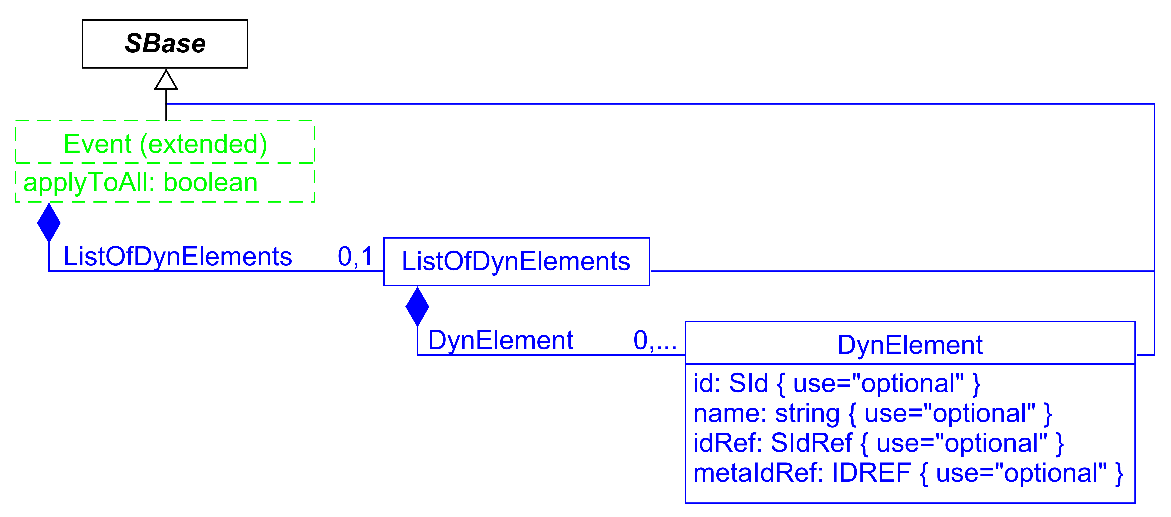
\includegraphics[width=0.70\textwidth]{images/UMLExtendedEvent.pdf}\\
  \caption{A UML representation of the extended \Event class and newly defined \ListOfElements and \Element objects. See \ref{subsec:conventions} for conventions related to this figure.} \label{fig:UMLExtendedEvent}
\end{figure}

\subsubsection{The \token{cboTerm} attribute}
\label{attr:cboTerm}

The attribute called \token{cboTerm} on the \Event class supports the use of Cell Behavior Ontology(CBO) terms to provide semantic encoding of dynamic cellular events in SBML models. By adding CBO terms, modelers can semantically annotate event constructs to explicitly indicate which cellular process is being modeled by each \Event instance. The relationship is of the form "the Event is-a X", where X is the CBO term. The term chosen should be the most precise one that captures the role of the Event in the model. The value of \token{cboTerm} must conform to the syntax permitted by the \primtype{CBOTerm} data type previously described in \sec{dat:CBOTerm} of the current specification. The scope of the \token{cboTerm} attribute is local to the enclosing object definition and is not visible outside the object definition. For a discussion on supported values for \token{cboTerm} and CBO in general see \sec{sec:CBO}

\subsubsection{The \token{applyToAll} attribute}
\label{attr:applyToAll}
The \token{applyToAll} attribute is used as a mechanism for indicating which SBML model components are impacted by the execution of the current dynamic \Event. If the value of this attribute is \val{true}, then all SBML elements in the model are involved in the \Event. If \val{false}, modelers must list the specific components that are affected by means of the \ListOfElements class, which must not be empty if present. For instance, if the value of the \token{cboTerm} attribute semantically annotates the current \Event as modeling cell death, the \token{applyToAll} attribute allows modelers to chose whether only some or all of the model components are to be removed from the simulation. 

\subsubsection{The \class{ListOfElements} class}
\label{subsec:ListOfElements}
An extended \Event component with \val{false} as value for its \token{applyToAll} attribute must define a non-empty object of class \ListOfElements. This object contains a list of \Element references that uniquely identify the set of SBML components involved in the execution of a given dynamic \Event.

\subsection{The \class{Element} class}
\label{subsec:Element}
An \Element object contains unique references to SBML components defined within a model. These references are pooled by a \ListOfElements construct and modified characteristically depending on the cellular process that is modeled. This construct defines an \token{element} attribute which stores a single reference to a given SBML model component.

\subsubsection{The \token{element} attribute}
\label{attr:element}

\token{Element} is a mandatory attribute of the type \primtype{SIdRef} that is used to reference single anatomical structures (compartments or submodels) or additional SBML components that are altered following the execution of a given dynamic event. Only model elements having identifiers of type \primtype{SId} can be referenced by this attribute. 

When \token{element} points to \Compartment element, it is advisable to define a \ListOfCoordinateComponents as seen in \ref{subsec:extCompartment}. This ensures that when an extended \Event is executed, referenced cellular compartments will have an assigned spatial location, which is important in representing dynamic behavior. On the other hand, if this attribute points to the identifier of a group from the SBML Groups extension, an \Element references not a single component, but a set of SBML objects instead. For a complete description of how \Element class instances are affected by different behaviors modeled in an extended \Event, refer to \sec{subsubsec:supportedCBO}.

{\color{red} Harold: \notice Are there any SBML components that won't be able to be referenced given the SIdRef type restriction?}

\subsection{The extended \class{Compartment} object}
\label{subsec:extCompartment}

The \Compartment class may be extended to represent the spatial location and subsequent rearrangement that follows dynamic cellular processes emulated by extended \Event constructs. Refer to \sec{sec:CBO} for a list of supported dynamic cellular processes and associated ontological terms. This SBML extension adds to \Compartment the subobjects \ListOfCoordinateComponents and \CoordinateComponent to describe the spatial location of cellular components. \ref{fig:UMLExtendedCompartment} provides the corresponding UML diagram of the various features of the extended \Compartment class. 

{\color{red} Harold: \notice If we add a rotation attribute here to support representations (bacterial growth) where rotation is important in spatially describing objects, it should be as 3 optional params of type SIdRef corresponding to rotations along the x, y, and z axes.}

\begin{figure}[tbhp]
	\centering
	%\usepackage{graphicx}
	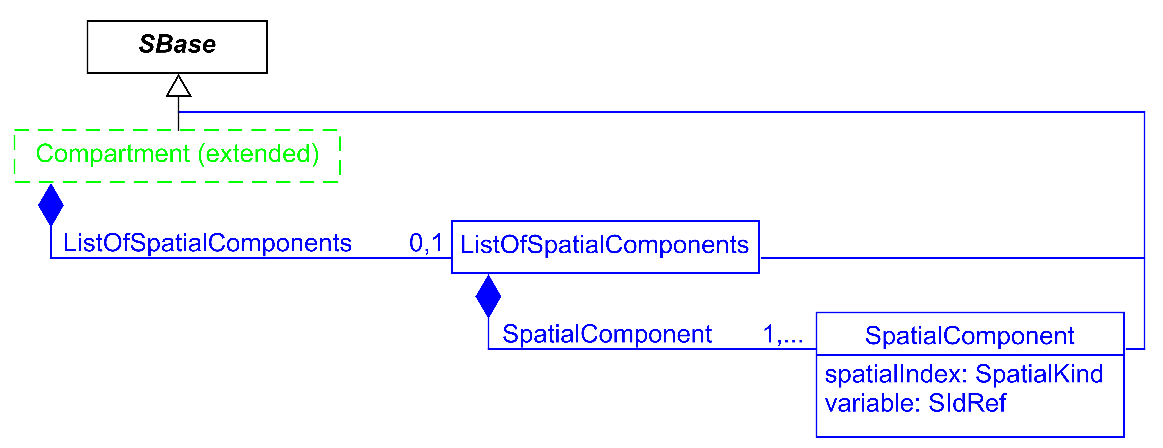
\includegraphics[width=0.85\textwidth]{images/UMLExtendedCompartment.pdf}\\
	\caption{UML diagram for the extension of the \Compartment object and the definition of \ListOfCoordinateComponents and \CoordinateComponent classes. See \ref{subsec:conventions} for conventions related to this figure.} \label{fig:UMLExtendedCompartment}
\end{figure}

{\color{red} Harold: \notice  Do we expect to model something of higher dimensions than 3D cartesian coordinate system?}

\subsubsection{The \class{ListOfCoordinateComponents} class}
\label{subsec:listCoordComp}

\Compartments mapped by an \Element construct may contain a listOfCoordinateComponents element, of class \ListOfCoordinateComponents. Each list contains \CoordinateComponent objects that together describe the spatial location (center of mass along a Cartesian coordinate system) of an individual \Compartment. If mapped, a \Compartment cannot have an empty \ListOfCoordinateComponents list.

\subsection{The \class{CoordinateComponent} class}
\label{subsec:coordComp}

Instances of the \CoordinateComponent class represent individual coordinate components of the spatial location of mapped \Compartment structures that are involved in dynamic events. This construct defines two attributes: \token{coordinateIndex} and \token{variable}. Being derived from SBase, this class also has all the usual attributes and elements of its parent class.

{\color{red} Harold: \notice So far we've defined the coordinate system and components to each x,y,z triplet for all compartments involved but nowhere have we defined the minimum and maximum values of the coordinate axis along which objects are modeled.
}

\subsubsection{The \token{coordinateIndex} attribute}
\label{attr:coordIndex}

The attribute \token{coordinateIndex} of type \primtype{CoordinateKind} is added to uniquely identify a coordinate axes in the defined \token{coordinateSystem}. \token{CoordinateIndex} may take one of all the possible \primtype{CoordinateKind} values specified in \sec{dat:CoordKind}. A single \val{cartesianX} \CoordinateComponent can be used to define one-dimensional systems; two-dimensional systems are in turn characterized by having two \CoordinateComponent children with \token{coordinateIndex} values of \val{cartesianX} and \val{cartesianY}; and three-dimensional ones can be defined by having three \CoordinateComponent elements with \token{coordinateIndex} values of \val{cartesianX}, \val{cartesianY}, and \val{cartesianZ}. 

\subsubsection{The \token{variable} attribute}
\label{attr:variable}

The \token{variable} attribute of type \primtype{SIdRef} contains the identifier of a \Parameter defined in the model to explicitly specify an object's position. The scope of the referenced \Parameter component must be global to the whole model and its \token{constant} attribute must be set to \val{false} as spatial location of the associated \Compartment may change in response to dynamic processes.
